\documentclass[a4paper, titlepage]{article}
\usepackage[round, sort, numbers]{natbib}
\usepackage[utf8]{inputenc}
\usepackage{amsfonts, amsmath, amssymb, amsthm}
\usepackage{color}
\usepackage{listings}
\usepackage{mathtools}
\usepackage{paralist}
\usepackage{parskip}
\usepackage{subfig}
\usepackage{tikz}
\usepackage{titlesec}

\numberwithin{figure}{section}
\numberwithin{table}{section}

\usetikzlibrary{arrows, automata, backgrounds, petri, positioning}
\tikzstyle{place}=[circle, draw=blue!50, fill=blue!20, thick]
\tikzstyle{marking}=[circle, draw=blue!50, thick, align=center]
\tikzstyle{transition}=[rectangle, draw=black!50, fill=black!20, thick]

% define new commands for sets and tuple
\newcommand{\setof}[1]{\ensuremath{\left \{ #1 \right \}}}
\newcommand{\tuple}[1]{\ensuremath{\left \langle #1 \right \rangle }}
\newcommand{\card}[1]{\ensuremath{\left \vert #1 \right \vert }}

\makeatletter
\newcommand\objective[1]{\def\@objective{#1}}
\newcommand{\makecustomtitle}{%
	\begin{center}
		\huge\@title \\
		[1ex]\small Dimitri Racordon \\ \@date
	\end{center}
	\@objective
}
\makeatother

\begin{document}

  \title{Outils formels de Modélisation \\ 5\textsuperscript{ème} séance d'exercices}
  \author{Dimitri Racordon}
  \date{20.10.17}
	\objective{
    Dans cette séance d'exercices,
    nous allons étudier les graphes de marquages
    et leurs relations avec les propriétés des réseaux de Petri
  }

	\makecustomtitle

\section{A la main?! ($\bigstar\bigstar$)}

Récupérez le fichier \texttt{MarkingGraph.swift} du répertoire \texttt{ex-05}, sur le dépôt GitHub.
Considérez le réseau de Petri de la figure \ref{fig:mutex}
et répondez aux questions suivantes:

\begin{enumerate}
  \item Combien d'états sont accessibles depuis le marquage initial?
  \item Le réseau est-il vivant?
  \item Encodez le graphe de marquage correspondant au réseau
        à l'aide de la classe \texttt{MarkingGraph} fournie.
\end{enumerate}

\begin{figure}[ht]
  \centering
  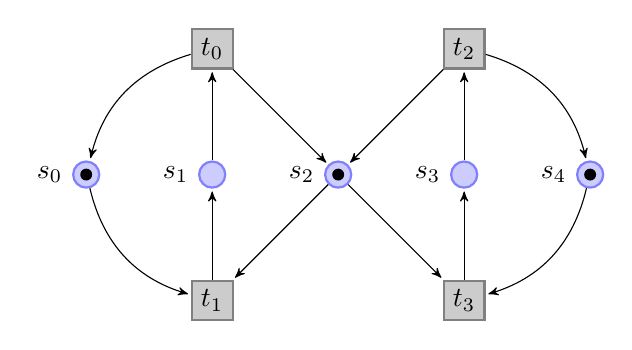
\begin{tikzpicture}[node distance=16mm, >=stealth', auto]
    \node[place,tokens=1] (s0) [label=left:$s_0$] {};
    \node[place] (s1) [right of=s0, label=left:$s_1$] {};
    \node[place,tokens=1] (s2) [right of=s1, label=left:$s_2$] {};
    \node[place] (s3) [right of=s2, label=left:$s_3$] {};
    \node[place,tokens=1] (s4) [right of=s3, label=left:$s_4$] {};

    \node [transition] (t0) [above of=s1] {$t_0$}
          edge [pre] (s1)
          edge [post,bend right] (s0) edge [post] (s2);
    \node [transition] (t1) [below of=s1] {$t_1$}
          edge [pre,bend left] (s0) edge [pre] (s2)
          edge [post] (s1);

    \node [transition] (t2) [above of=s3] {$t_2$}
          edge [pre] (s3)
          edge [post,bend left] (s4) edge [post] (s2);
    \node [transition] (t3) [below of=s3] {$t_3$}
          edge [pre,bend right] (s4) edge [pre] (s2)
          edge [post] (s3);
  \end{tikzpicture}
  \caption{Une exclusion mutuelle simple}
  \label{fig:mutex}
\end{figure}

\section{Nodes, nodes everywhere ... ($\bigstar\bigstar\bigstar$)}

Récupérez le fichier \texttt{MarkingGraph.swift} du répertoire \texttt{ex-05}, sur le dépôt GitHub.
Ce fichier contient plusieurs graphes de marques,
encodés à la main.
Notez qu'on considère le noeud nommé \texttt{m0} comme le marquage initial.
Pour chacun de ces graphes, répondez aux questions suivantes:

\begin{enumerate}
  \item Combien d'états sont accessibles depuis le marquage initial?
  \item Déssinez le réseau de Petri correspondant au graphe?
  \item Le réseau est-il vivant?
\end{enumerate}

\end{document}
